\documentclass[12pt]{article}
\usepackage[a4paper, portrait, margin=2cm]{geometry}
\usepackage{graphicx} % Required for inserting images
\usepackage[page,toc,titletoc,title]{appendix}
\usepackage{mathptmx}
\usepackage{pdflscape}
\usepackage{pdfpages}
\usepackage{enumitem}
\usepackage{hyperref}
\usepackage{cleveref}
\usepackage{wrapfig}
\usepackage{gensymb}
\usepackage{amssymb}
\usepackage{makecell}
\usepackage{pifont}% http://ctan.org/pkg/pifont
\usepackage{listings}
\usepackage{xcolor}
\usepackage{array}
\usepackage{ragged2e}
\newcommand{\cmark}{\ding{51}}%
\newcommand{\xmark}{\ding{55}}%
\newcolumntype{L}[1]{>{\RaggedRight\hspace{0pt}}p{#1}}
\newcolumntype{R}[1]{>{\RaggedLeft\hspace{0pt}}p{#1}}


\definecolor{codegreen}{rgb}{0,0.6,0}
\definecolor{codegray}{rgb}{0.5,0.5,0.5}
\definecolor{codepurple}{rgb}{0.58,0,0.82}
\definecolor{backcolour}{rgb}{0.95,0.95,0.92}

\lstdefinestyle{mystyle}{
    backgroundcolor=\color{backcolour},   
    commentstyle=\color{codegreen},
    keywordstyle=\color{magenta},
    numberstyle=\tiny\color{codegray},
    stringstyle=\color{codepurple},
    basicstyle=\ttfamily\footnotesize,
    breakatwhitespace=false,         
    breaklines=true,                 
    captionpos=b,                    
    keepspaces=true,                 
    numbers=left,                    
    numbersep=5pt,                  
    showspaces=false,                
    showstringspaces=false,
    showtabs=false,                  
    tabsize=2
}

\lstset{style=mystyle}


\title{Building Digital Twins on Existing Infrastructure: Evaluating The Effectiveness of IDAES for Live Data Processing}

\author{Bert Downs\\
\textit{Ahuora Research Group}\\
\textit{University of Waikato}\\
\textit{Hamilton, New Zealand}\\
\texttt{bd65@students.waikato.ac.nz}}

\date{October 2024}

\begin{document}

\maketitle

\section*{Abstract}
% A concise and factual abstract is required. The abstract should state briefly the purpose of the research, the principal results and major conclusions. An abstract is often presented separately from the article, so it must be able to stand alone. For this reason, References should be avoided, but if essential, then cite the author(s) and year(s). Also, non-standard or uncommon abbreviations should be avoided, but if essential they must be defined at their first mention in the abstract itself.


Digital Twin technology promises improvements in factory performance by optimising based on a digital model that updates to follow physical conditions. This research evaluates the IDAES Process Simulation Environment for use in developing Digital Twins, to show that it can provide for many of the core requirements of a Digital Twin. A theoretical framework is presented to generalise the concept of a Digital Twin. The framework shows that a Digital Twin can be viewed as a software system built on top of an existing simulation platform and live data processing system. 

% Keywords. Immediately after the abstract, provide a maximum of 6 keywords avoiding general and plural terms and multiple concepts (avoid, for example, "and", "of"). Be sparing with abbreviations: only abbreviations firmly established in the field may be eligible. These keywords will be used for indexing purposes.


\begin{center}
\textbf{Keywords:} Digital Twin; IDAES-PSE; Process Simulation; Hybrid Modelling
\end{center}

\subsection*{List of Abbreviations}
\begin{tabular}{lL{13cm}}
    IDAES-PSE & Institute for the Design of Advanced Energy Systems - Process Simulation Environment \\
    SCADA & Supervisory Data Aquisition and Control \\
    ODE & Ordinary Differential Equation \\
    PDE & Partial Differential Equation \\
    RBF & Radial Basis Function \\
    PYSMO & Python-based Surrogate Modelling Objects \\
    OMLT & Optimization and Machine Learning Toolkit \\
\end{tabular}

\section{Introduction}
% State the objectives of the work and provide an adequate background, avoiding a detailed literature survey or a summary of the results.


Traditional factory control systems are based on feedback loops that use sensor data to adjust the factory's state. 
However, these systems are limited in their ability to predict future states and optimise factory performance. 
Digital Twinning is a new approach that combines live factory data, historical state, mathematical modelling, and data-driven modelling to create a digital replica of the factory. 
Yet in existing literature, most examples of digital twinning focus on specific situations rather than providing a general framework for creating digital twins.
Many remain at the proof-of-concept stage, and have not yet been deployed in industrial settings.

In order to implement digital twinning in industry, simulation platforms must be able to work with and process live data, but most simulation environments are designed for design and analysis, rather than real-time processing \cite{agi2024computational}. The objective of this research is to evaluate how effectively an existing simulation platform can be used or extended to process live data.

One such simulation platform is the IDAES-PSE modelling framework, which is designed for the analysis of chemical processes \cite{lee2021idaes}. 
It supports a variety of modelling techniques, including steady-state chemical modelling, and dynamic modelling of time-dependent processes. 
It has also been extended to support data-driven modelling techniques, using libraries such as PySMO and OMLT \cite{cecconOMLTOptimizationMachine2022} 


This research evaluates the extent to which the IDAES-PSE modelling framework can be used to implement emerging chemical modelling techniques for live data processing, to prove it's suitability as a platform on which to develop such tools.
The results of this research are used to propose a general framework for implementing digital twinning in industry.


\section{Theoretical Framework}\label{sec:theoretical_framework}

Conventional simulation platforms do not have built-in support for live data processing. Likewise, conventional factory SCADA\footnote{SCADA systems: Supervisory Data Aquisition and Control systems.} systems do not have built-in support for complex simulation. To integrate a simulation platform with live data, a software system must be created that can merge the two systems. This can be considered as an intermediate layer between the simulation platform and the factory SCADA system.


% Todo: Should this be generalised further, removing references to specific model types for a simulation platform an a factory floor environment? (I.e don't list steady state modelling etc, data collection etc)
% Then, in the discussion section, the specific implementation of these can be added.
\begin{figure}[h]
    \centering
    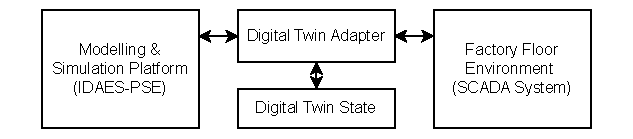
\includegraphics[width=0.7\textwidth]{research_journal_framework_simple.pdf}
    \caption{Theoretical framework for evaluating IDAES-PSE in a live data processing context.}
    \label{fig:theoretical_framework}
\end{figure}

The concept of a “Digital Twin” refers to a simulation of something in the physical world, which is kept up to date with a physical system using real-time data \cite{yu2022energy}.
In \cref{fig:theoretical_framework}, this intermediate layer is what converts the simulation platform, and the data from the factory, into a digital twin. It is broken into two parts: a ``Digital Twin Adapter'' which is responsible for converting the data from the factory into a format that the simulation platform can understand, and to provide results from simulations back the factory. Also specified is a ``Digital Twin State'', which represents an estimate of the current state of the factory, based on the simulation results and the live data. This represents the ability of a Digital Twin to "learn" how the physical system behaves, and adjust the inputs to the simulation accordingly.

The results of evaluating the IDAES-PSE platform will be considered in the context of this theoretical framework, to determine what the high-level requirements are for a Digital Twin that is built on top of existing simulation and live data processing platforms.

\subsection{Limitations of Live Data Processing} \label{sec:limitations_framework}

% TODO: Citations needed

The Digital Twin intermediate layer will be working with live data, which adds additional engineering constraints. There is no access to any future data, so the system must only use data that is available at the time of prediction. Live data can also be noisy, delayed, or missing, so the system must be robust enough to handle these situations. Additionaly, there is a time constraint on processing the data, as the system must be able to respond to changes in the factory in real-time. Practically, this means that there is only a window of recent data that can be used at any point in time, unless aggregation or smoothing techniques are used.

\section{Method}
%Experimental procedure
%Provide sufficient details to allow the work to be reproduced by an independent researcher. Methods that are already published should be summarized, and indicated by a reference. If quoting directly from a previously published method, use quotation marks and also cite the source. Any modifications to existing methods should also be described.
%This section can contain Material and methods and Theory/calculation. A Theory section should extend, not repeat, the background to the article already dealt with in the Introduction and lay the foundation for further work. In contrast, a Calculation section represents a practical development from a theoretical basis.

IDAES has many components, so an iterative validation process is used. The evaluation is broken down into parts, each focusing on a different piece of functionality. 

The core functionality of the IDAES modelling framework is steady-state modelling, where a chemical system is in a stable equilibrium and variables do not change over time. In a live data processing context, steady-state simulations can be used to model the entire state of the factory, based on a sample of avaliable sensor data. Multiple steady-state simulations can be run at different time steps, but each represents a stable equilibrium. This is the simplest form of modelling to integrate with live data. 

\begin{table}[h]
    \centering
    \begin{tabular}{|l|p{10cm}|}
        \hline
        \textbf{Functionality} & \textbf{Description} \\
        \hline
        Steady State Modelling & Analysis of systems in a stable equilibrium where variables do not change over time. \\
        \hline
        Dynamics & Modelling of time-dependent processes to understand how systems evolve over time. \\
        \hline
        Optimisation/Control & Techniques to find the best operating conditions or control strategies for a system. \\
        \hline
        Hybrid Modelling & Combining different modelling approaches, such as data-driven and first-principles models, to improve accuracy and robustness. \\
        \hline
    \end{tabular}
    \caption{Different pieces of functionality evaluated from the IDAES-PSE framework.}
    \label{tab:functionality}
\end{table}

Dynamic Modelling adds a time dimension to the simulation, allowing changes in the system to propogate through over time. This is useful for predicting how a factory will respond to changes in input conditions, and can be a key decision-making tool for factory operators.

Optimisation and Control techniques can be used to find the best operating conditions for a system, or to develop control strategies that keep the system in a desired state. This enables closed-loop control of a industrial process, where the system can automatically adjust itself to maintain optimal conditions.

Hybrid Modelling implements Machine Learning techniques into the model. IDAES is built on Pyomo, an algebraic modelling language \cite{bynum2021pyomo}, but it is possible to combine machine learning techniques with data-driven modelling libraries such as PySMO. 
This is useful for situations where the system is too complex to model using a single approach, or where data is available but the underlying physics are not well understood for parts of the system. 
The aim of hybrid modelling is to increase generalisation and explainability compared to purely data-driven models, and increase accuracy and adaptability compared to purely first-principles models.


For each of piece of functionality listed in \cref{tab:functionality}, a simple prototype flowsheet is developed to evaluate the functionality of IDAES-PSE in a live data processing context. This flowsheet consists of a Heater, that is heating steam from an inlet temperature of approximately 600 K at atmospheric pressure. This approach allows to focus on the functionality of the IDAES-PSE framework, rather than the complexity of the flowsheet, as the techniques used generalise to larger and more complex systems.


\subsection{Evaluation Criteria}

Each functionality is tested using by developing and evaluating a simple prototype in the IDAES-PSE framework. 

The prototypes are used to evaluate the functionality of IDAES-PSE against three broad categories of use in a factory floor environment: As a standalone tool, when connected with process data, and when connected to control systems. 

\begin{table}[h]
    \centering
    \begin{tabular}{|l|p{10cm}|}
        \hline
        \textbf{Category} & \textbf{Evaluation Criteria} \\
        \hline
        As standalone tools & How well does IDAES-PSE perform the functionality on its own? \\
        \hline
        With process data & Are the tools useful to better process data from a factory? What additions or modifications are needed to make them useful? \\
        \hline
        For control systems & Can the tools be used to improve control systems in a factory? What  is required to do so? \\
        \hline
    \end{tabular}
    \caption{Evaluation criteria for IDAES-PSE functionality.}
    \label{tab:evaluation_criteria}
\end{table}

Evaluating the functionality of IDAES-PSE as a standalone tool gives an indication of the core functionality. This acts as a control, to compare what value is added when connected with live data systems. It acts as an indication of what IDAES functionality is useful for conventional process modelling.

Analysing how the functionality can be used with process data and control systems gives an indication of the potential value of simulation software in a factory environment. This is used to systematically explore a range of potential use cases for simulation software. 
To do this, some sample data is generated, and then different techniques are used to process the sample data, emulating how live data would be used in a factory environment.

The evaluation criteria do not focus on the accuracy of the IDAES platform in performing chemical simulations, or user-friendliness of the interfaces, or the performance of the solving process itself. Those characteristics are considered out of scope of this study, and are evaluated elsewhere \cite{hart2011pyomo} \cite{myhre2022investigation}. Instead, the evaluation criteria focus on the ability of the IDAES platform to be used for live data processing, and the ease of integration with other systems.



%Process Data
%Maintenance Data
%Control Systems
% Manual control






\section{Steady State Modelling} \label{sec:steady_state}

\begin{table}[h]
    \centering
    \begin{tabular}{|l|c|}
        \hline
        \textbf{Property} & \textbf{Value} \\
        \hline
        Inlet Flow (mol/s) & 100 , \\
        \hline
        Inlet Temperature (K) & 380 , \\
        \hline
        Inlet Vapor Fraction & 1 ,  \\
        \hline
        Inlet Pressure (Pa) & 101325 ,  \\
        \hline
        Heat Duty (J) & 100,000 , \\
        \hline
    \end{tabular}
    \caption{Specified properties of the heater.}
    \label{tab:heater_properties}
\end{table}

A simple heater model is developed in IDAES, with the properties specified in \cref{tab:heater_properties}. The model is then solved to find the outlet temperature.

\begin{lstlisting}[language=Python,caption=Defining a simple heater model in IDAES,label=lst:heater_model]
m.fs.heater = Heater(property_package=m.fs.properties)

m.fs.heater.inlet.flow_mol[0].fix(100)
m.fs.heater.inlet.temperature[0].fix(380)
m.fs.heater.inlet.vapor_frac[0].fix(1)
m.fs.heater.inlet.pressure[0].fix(101325)
m.fs.heater.heat_duty[0].fix(100_000)

solver = pyo.SolverFactory("ipopt")
solver.solve(m)

\end{lstlisting}

As shown in Listing \ref{lst:heater_model}, IDAES-PSE enables a declarative approach to defining models. IDAES is built on top of Pyomo, an algebraic modelling language, which allows for the use of Pyomo's solver interfaces to solve the model. IDAES provides the equations for the thermodynamic and chemical properties of materials and unit operations. IDAES provides a time set for simulation, and the user can specify at what time steps the model will be solved. However, without enabling dynamic modelling, these time steps are independent. In Listing \ref{lst:heater_model}, the model is solved at only a single steady state.

This model can be easily extended to solve multiple steady-state systems, however, they would be all solved as a single batch by IPOPT. In a live data processing context, this would not be useful, because the model needs to be solved for each new set of sensor data when the data is received. 

Because IDAES is built in Python, a model can easily be incorporated into a script that reads new data from a stream, and then solves the model with the new data. 

\begin{figure}
    \centering
    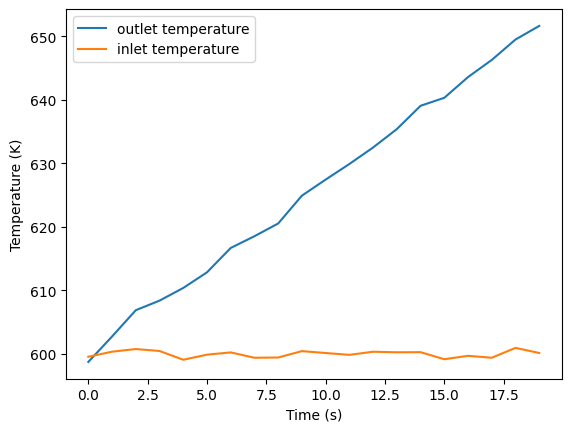
\includegraphics[width=0.6\textwidth]{live_data_processing.png}
    \caption{Solving a steady-state model with mock sensor data.}
    \label{fig:live_mss}
\end{figure}

To prove this, a simple script is developed that generates mock sensor data for the heater model. The mock data includes inlet temperatures, which is varied randomly between 599 and 601 K, and inlet pressures, which is set to be approximately 101325 Pa, with a random noise of 5 Pa. A ramp in power from 0W to 20,000W is applied over 20 seconds. The model is then solved with this data, and the outlet temperature is plotted over time. This is shown in \cref{fig:live_mss}. At each time step, the model is solved with the most recent sensor data, to provide an estimate of the conditions.


\subsection{Evaluation}


Steady-state modelling is the core functionality of IDAES. Developing this type of model is well-documented and supported, and solving is robust as long as the model is built with physically feasible conditions.
It would be possible to use a steady-state idaes model in a live data processing context, if it was integrated into a process toolchain. Because IDAES has a standardised way of presenting unit models, a data processing framework for multi-steady state can be built in Python that is seperate to the IDAES model itself, but can be linked with any IDAES model.

This would enable modelling live conditions in a factory that are not directly measurable, such as the state of a chemical reaction, or the state of a material in a process. Control systems could use this data to estimate how close the system is to the ideal state, and adjust the system to maintain optimal conditions.



\section{Dynamics}

To evaluate Dynamic modelling in IDAES-PSE, the heater model is extended to include holdup. Holdup is a property that represents how long it takes for changes to propogate through the system. The heater is modelled over 1 second, with the heat duty instentaneously changing from 0 to 10,000 W half a second through the simulation. As shown in \cref{fig:dynamic_test}, the outlet temperature change is not modelled as an instantaneous change, but instead propogates through the system over time.

\begin{figure}
    \centering
    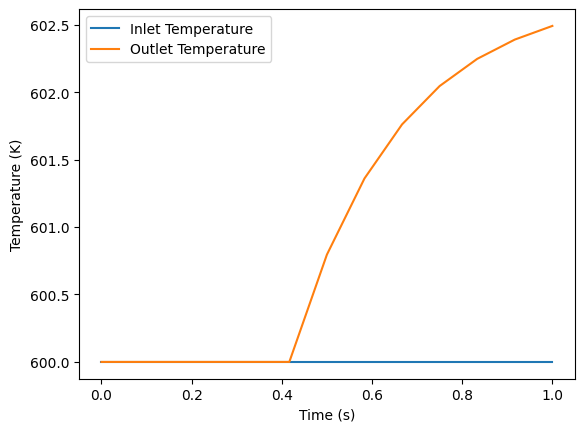
\includegraphics[width=0.8\textwidth]{dynamic_test.png}
    \caption{Solving a dynamic model with mock sensor data.}
    \label{fig:dynamic_test}
\end{figure}

This technique could be used in a live system to predict how the system will respond to a change in input conditions. This is particularly valuable in a factory environment, where changes in input conditions can have a significant impact on the system, and may take a long time to propogate through the entire system. \cite{CITATION_NEEDED}

% Why was this other model created?
To show how a dynamic model could be used in a live data processing context, the same sample data used in \cref{sec:steady_state} is used in a dynamic model. In steady-state, there is no time dimension, so each timestep can be solved seperately. In Dynamic modelling, all timesteps must be solved together. The inlet conditions are specified exactly the same as in the steady state example, but are interpolated between time steps. 

\begin{figure}
    \centering
    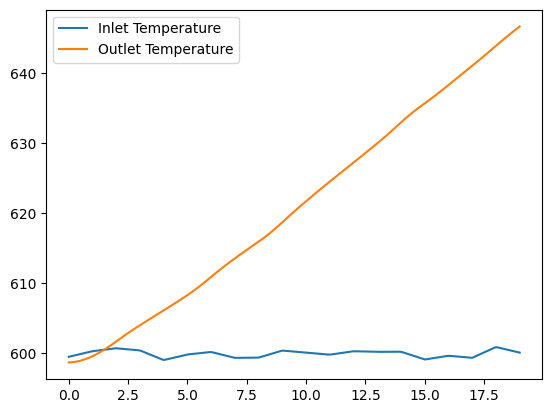
\includegraphics[width=0.7\textwidth]{dynamic_live.png}
    \caption{Solving a dynamic model with mock sensor data.}
    \label{fig:dynamic_live}
\end{figure}

In \cref{fig:dynamic_live}, a smoothing effect is observed in comparison to the steady-state model in \cref{fig:live_mss}. This is because it takes time for changes to propogate through. In chemical and process engineering, dynamic models provide a more accurate representation of how a system will respond to change. \cite{CITATION_NEEDED}


\subsection{Evaluation}
% explain why it is/isnt complete as a standalone tool
The IDAES framework is well-suited to dynamic modelling, as it provides tools for creating and solving differential equations. It can easily model the same system at different time scales. Dynamic models certainly are much more complex than steady-state models, but IDAES and Pyomo provide the tools to handle this complexity.

Mathematically, dynamic modelling is solving an ODE or PDE system, breaking it into a set of finite elements, and then solving the resulting algebraic equations. This means that each time step cannot be calculated completely independently of the previous time step.

In a live data processing context, this makes is more complex to run dynamic models. 
However, the problem can still be formulated using only past data, so it is possible to use dynamic models in a live data processing context.
The final conditions of one time step (variables, and their derivatives) must be used as initial conditions of the next time step. This will contribute to the ``State'' of the Digital Twin as outlined in \cref{sec:theoretical_framework}.

Additionally, the model may need to be discretised between time steps to provide a more accurate continuous solution. This will involve interpolating betweeen data points from the factory, or estimating missing values.


Dynamic models can also be used for predicting future states. However, new data will require that all subsequent time steps be recalculated. 
If the model and initial conditions are specified correctly, from a software development perspective this is no more complex to implement than a steady state model, but it is much more computationally expensive to solve. 
.

\section{Optimisation}
Optimising a system involves adding an objective the model using standard Pyomo utilities, and then solving the model to find the optimal conditions. In the heater model, a cost function is added as a test objective, to find the ideal balance between heat duty and outlet temperature. The model is then solved to find the optimal heat duty that minimises the cost function.

\begin{lstlisting}[language=Python,caption=Optimising the heater model in IDAES,label=lst:optimisation]
def cost_objective(h):
return 3**(h.heat_duty[0]/5000) - (h.outlet.temperature[0]-350) * 33000
m.fs.heater.cost_objective = pyo.Objective(rule=cost_objective, 
                                           sense=pyo.minimize)
\end{lstlisting}

This is shown in Listing \ref{lst:optimisation}. The model must be solved with degrees of freedom, i.e variables that the solver can adjust to find the optimal solution. In this case, the heat duty is the degree of freedom, but there can be multiple degrees of freedom in a model. 
In \cref{fig:optimisation_dynamics}, a setpoint function for the outlet temperature is added, and optimisation is used to find the heat duty for each timestep that best follows the setpoint. This has one degree of freedom for each discrete time step that must be optimised: the heat duty at that time step. 
Because the setpoint change is instantaneous, it is unable to perfectly follow the setpoint, but is able to minimise the error on either side of the setpoint. 
This  can be used in a live data context for model predictive control.\cite{CITATION_NEEDED}

\begin{figure}
    \centering
    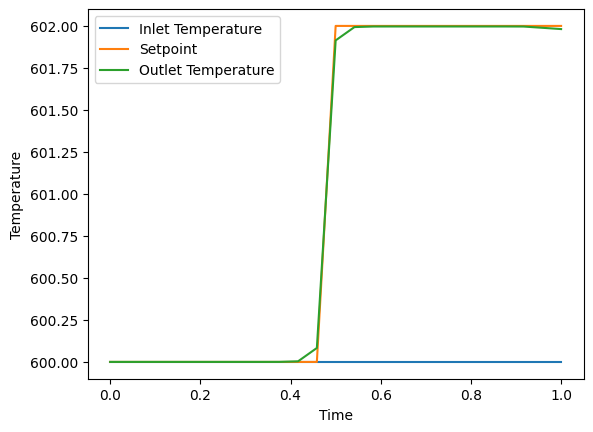
\includegraphics[width=0.7\textwidth]{dynamics_optimisation.png}
    \caption{Optimising a dynamic model to follow a setpoint.}
    \label{fig:optimisation_dynamics}
\end{figure}


\subsection{Evaluation}


Because optimisation has first-party support from Pyomo, it is well-supported as a standalone tool, and well integrated with IDAES.  It can be used for control to find the optimal setpoints to use. The optimising functionality is generic, so it can also be used for other types of optimisation, such as predicting the most likely conditions from uncertainty (though Pyomo has additional tools to support this that are not considered as part of this study.)

IDAES also supports multi-level modelling, and because it is built on an algebraic modelling language it is possible to include other variables in the optimisation, such current energy costing figures. More advanced models could include these factors, without sigificant rework of the Digital Twin system.

% TODO: What else is required to talk about this?

\section{Hybrid Modelling}

To test the workflow for hybrid modelling, a simple surrogate model is created using PySMO. First, a set of data points is generated by solving a heater model at different pressures, temperatures, and flow rates. 
Then, this data is used to train a surrogate model, which can predict the outlet pressure and enthalpy from the valve based on the inlet conditions. 
This generated data for a steady-state simulation, predicting the outlet pressures and temperatures. 
An RBF\footnote{Radial Basis Function} network is trained to predict these values from the inlet conditions.
The weights of the trained model are then saved to disk. 

% TODO: To use them in a model ..
To use the surrogate model in a flowsheet, the weights of the model are loaded and the structure of the model is recreated as a set of algebraic constraints, relating the input conditions to the predicted output conditions. This can be combined with IDAES's UnitModel class and StateBlocks to create a new unit operation that can be used in a flowsheet.


\begin{figure}
    \centering
    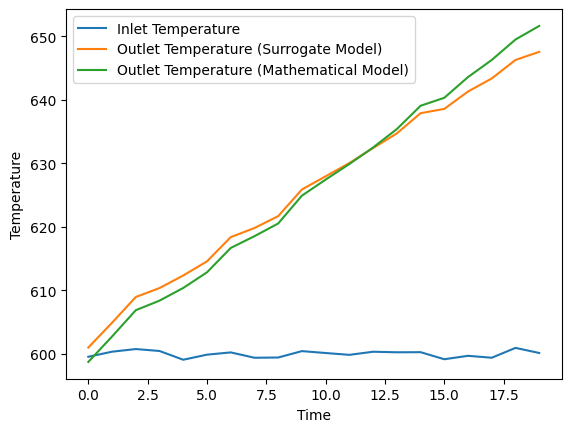
\includegraphics[width=0.6\textwidth]{surrogate_model_accuracy.png}
    \caption{Comparison of the output of the surrogate model and the IDAES mathematical model.}
    \label{fig:surrogate_model}
\end{figure}

In \cref{fig:surrogate_model}, the output of the surrogate model is compared to the output of the IDAES model. The surrogate model is able to closely follow the IDAES mathematical model, but it does not match exactly. For the purposes of this demonstration, the accuracy is not important; with careful tuning of the surrogate model, it is possible to get a very close match to the IDAES model. However, in a live data processing context, the surrogate model could be retrained using recent process conditions, deviating from the mathematical solution to better reflect real-world nuances in the system. 

This demonstration uses a simple RBF network, but other machine learning techniques can also be used, as long as there is support for creating algebraic constraints to represent them in Pyomo. In theory, it is possible to model a dynamic system in the same way that this steady-state system is modelled, but there is less evidence of this being done in IDAES.

\subsection{Evaluation}

% explain it as a standalone tool

% Todo: Proofread this

Surrogate Modelling may be achieved using IDAES's built-in PySMO libraries, or other similar libraries such as OMLT. 
It is reasonably straightforward to train a surrogate model to represent a non-dynamic unit operation, but dynamic unit operations get significantly more complex - instead of modelling a single value, the surrogate model must be able to model the entire time system. There are some methods of doing this, such as using neural ODEs, Residual Networks, Operator Networks, or some other sort of convolutional network. 
There is little research into applying these methods in the field of chemical and process simulation, especially in the context of mathematical modelling such as the IDAES framework.

The exact same process for surrogate modelling can also be used to model unit operations from historical data. 
This is useful when there is no mathematical model of the unit operation, but there is historical data available. 
This would be very useful when applying the Ahuora Digital Twin Platform to existing factories, where the exact mathematical properties of the unit operations are unknown but there is a wealth of historical data available. 
Online Learning techniques could be used to update the surrogate model in real-time, as new data becomes available. This is a key step in turning a ``simulation" into a ``Digital Twin", as it allows the model to self-adapt to real-world conditions. The current machine learning libraries in IDAES do not support this, so this functionality would need to be added.



% for process data

% for control systems

\section{Results \& Discussion}
%Results should be clear and concise.
\subsection{Results}

The morphological matrix in \cref{tab:morphological_matrix} shows the discussed ways of where the IDAES-PSE functionality could be used in a factory environment. While IDAES-PSE provides the core simulation backend to support these use cases, the research into each functionality has proven that a custom software solution will be required to integrate it with live data systems.

\begin{table}[h]
    \centering
    \begin{tabular}{|p{2.4cm}|p{4cm}|p{4cm}|p{4.5cm}|}
        \hline
        \textbf{Functionality} & \textbf{As Standalone Tools} & \textbf{With Process Data} & \textbf{For Control Systems} \\
        \hline
        \makecell{Steady State \\ Modelling} & 
        Basic analysis of systems in equilibrium & 
        Model live conditions & 
        Estimate target conditions for control strategies \\
        \hline
        \makecell{Dynamics} & 
        Simulate how changes propogate across a system & 
        Predict effect of changing input conditions & 
        Develop dynamic control strategies \\
        \hline
        \makecell{Optimisation} & 
        Find optimal operating conditions & 
        Multi-Scale Global Optimisation & 
        Implementing Model Predictive control \\
        \hline
        \makecell{Hybrid \\ Modelling} & 
        Combine modelling approaches for better accuracy & 
        Online learning so digital twin matches physical state & 
        Self-Adaptive control systems based on past performance \\
        \hline
    \end{tabular}
    \caption{Morphological matrix showing overlaps and use cases of IDAES-PSE functionality.}
    \label{tab:morphological_matrix}
\end{table}
% Add another table showing the gaps of what needs to be implemented to make IDAES-PSE a complete Digital Twin platform.

%\subsection{Gaps in IDAES-PSE Functionality}
% \begin{table}[h]
%     \centering
%     \begin{tabular}{|L{3cm}|L{3.8cm}|p{8.5cm}|}
%         \hline
%         \textbf{Functionality} & \textbf{Gap} & \textbf{Explanation} \\
%         \hline
%         Steady State Modelling & 
%         System to solve with live data &
%         Aggregating live data measurements and passing them to the simulation\\
%         \hline
%         Dynamic Modelling & 
%         Data Interpolation & 
%         Estimating data in between sensor readings for a continuous simulation.\\
%         \hline
%         Dynamic Modelling &
%         Dynamic State &
%         Storing the final state of the dynamic system so it can be used as the initial state for the next timestep  \\
%         \hline
%         Optimisation & 
%         Model Predictive Control &
%         Implementing a model-predictive control system that can connect to a simulation platform such as IDAES-PSE, and give control signals to the factory. \\
%         \hline
%         Hybrid Modelling & 
%         Online learning & 
%         Creating a system to update models based on recently aquired sensor data. \\
%         \hline
%     \end{tabular}
%     \caption{Gaps in IDAES-PSE functionality for factory systems.}
%     \label{tab:gaps_functionality}
% \end{table}

\begin{figure}[h]
    \centering
    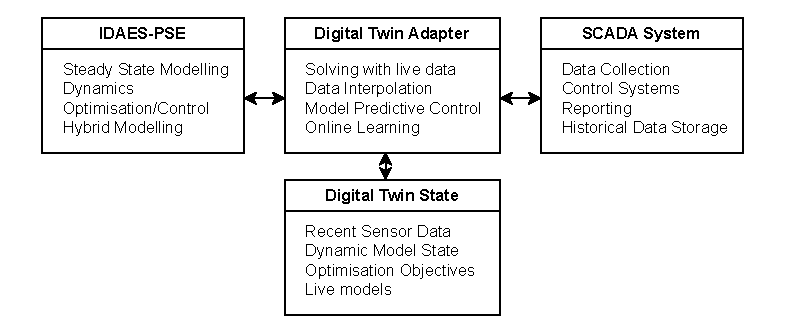
\includegraphics[width=0.95\textwidth]{research_journal_framework_full.pdf}
    \caption{Key Components of a Digital Twin system built on top of IDAES-PSE.}
    \label{fig:theoretical_framework_full}
\end{figure}

\Cref{fig:theoretical_framework_full} summarises what additional functionality would be required to communicate with a factory system. These can be viewed as the ``Digital Twin Adapter'' and ``Digital Twin State'' as outlined in \cref{sec:theoretical_framework}.

% Discussion
% This should explore the significance of the results of the work, not repeat them. A combined Results and Discussion section is often appropriate. Avoid extensive citations and discussion of published literature.
%Note: results and Discussion can also be combined in a single section.

\subsection{Discussion}

This analysis is unique among the field of Digital Twinning, as it looks at the problem from a software engineering perspective, and does not focus on a custom-built solution.

These results prove the effectiveness of IDAES-PSE as a platform for developing Digital Twins. It outlines how a general solution can be implemented on top of a simulation platform to turn it into a digital twin. The theoretical framework outlined can be used to evaluate other simulation platforms, and factory SCADA systems, to compare them to IDAES-PSE for a broader understanding of the problem space.

In a software context, this provides a set of requirements for such a software system to be developed on top of IDAES-PSE.
Development of such a general-purpose digital twin platform for process engineering would be a significant contribution to the field, as it would enable factories of all sizes to take advantage of the benefits of digital twinning.


\section{Conclusions}
% The main conclusions of the study may be presented in a short Conclusions section, which may stand alone or form a subsection of a Discussion or Results and Discussion section.

By seperating the simulation platform from the live data processing system, it is possible to create a general-purpose Digital Twin platform that can be used in a variety of factory environments.
The IDAES-PSE modelling framework is well-suited to developing Digital Twins for chemical processes. 
This is because it is supported by an algebraic modelling language, which easily lends it to extensibility and integration with other systems. Additionally, it's simulation techniques are relevant to live data processing.
With appropriately designed software, techniques from IDAES-PSE such as steady-state modelling, dynamic modelling, optimisation, and hybrid modelling can be used to analyse live data from a factory process. 
A software system that is built on top of this functionality would enable a much wider audience to take advantage of the benefits of digital twinning. 

\section*{Acknowledgements}
% Collate acknowledgements in a separate section at the end of the article before the references and do not, therefore, include them on the title page, as a footnote to the title or otherwise. List here those individuals who provided help during the research (e.g., providing language help, writing assistance or proof reading the article, etc.).

This research has been conducted as part of the development of the Ahuora Digital Twin Platform, a key project of the Ahuora Research Group. A sincere thanks to all those who have provided feedback and support during the writing of this paper, particularly many members of the Ahuora Research Group: Tim Walmsley, Mark Apperley, Stephen Burroughs, Ben Lincoln, and many others.

% References
% Please ensure that every reference cited in the text is also present in the reference list (and vice versa). Unpublished results and personal communications are not recommended in the reference list, but may be mentioned in the text. If these references are included in the reference list they should follow the standard reference style.
\bibliographystyle{apalike}
\bibliography{refs} % Entries are in the refs.bib file

% If there is more than one appendix, they should be identified as A, B, etc. Formulae and equations in appendices should be given separate numbering: Eq. (A.1), Eq. (A.2), etc.; in a subsequent appendix, Eq. (B.1) and so on. Similarly for tables and figures: Table A.1; Fig. A.1, etc.
% \begin{appendices}
% \end{appendices}


\end{document}